\usetikzlibrary{arrows}
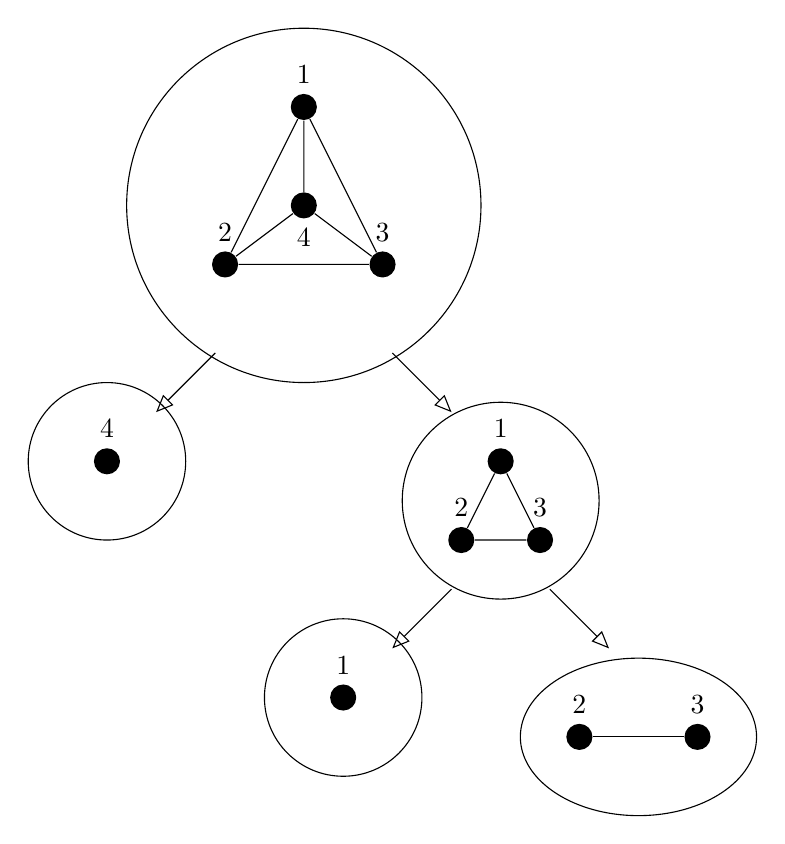
\begin{tikzpicture}





\node [fill, circle, label=1] (v2) at (-1.5,4) {};

\node [fill, circle, label=2] (v1) at (-2.5,2) {};

\node [fill, circle, label=3] (v3) at (-0.5,2) {};

\node [fill, circle, label=below:4] (v4) at (-1.5,2.75) {};

\draw (v1) -- (v2) -- (v3) -- (v1) -- (v4) -- (v2);

\draw  (v4) edge (v3);

\draw  (v4) ellipse (2.25 and 2.25);

\node (v5) at (-2.5,1) {};

\node (v6) at (-3.5,0) {};

\node (v7) at (-0.5,1) {};

\node (v8) at (0.5,0) {};

\draw [-open triangle 45] (v5) edge (v6);

\draw [-open triangle 45] (v7) edge (v8);



\node [fill, circle, label=4] (v9) at (-4,-0.5) {};



\draw  (v9) ellipse (1 and 1);

\node [fill, circle, label=1] (v10) at (1,-0.5) {};

\node [fill, circle, label=2] (v12) at (0.5,-1.5) {};

\node [fill, circle, label=3] (v11) at (1.5,-1.5) {};

\draw (v10) -- (v11) -- (v12) -- (v10);

\draw  (1,-1) ellipse (1.25 and 1.25);

\node (v13) at (0.5,-2) {};

\node (v15) at (1.5,-2) {};

\node (v14) at (-0.5,-3) {};

\node (v16) at (2.5,-3) {};

\draw [-open triangle 45] (v13) edge (v14);

\draw [-open triangle 45] (v15) edge (v16);

\node [fill, circle, label=1] (v17) at (-1,-3.5) {};
\draw  (v17) ellipse (1 and 1);




\node [fill, circle, label=2] (v18) at (2,-4) {};

\node [fill, circle, label=3] (v19) at (3.5,-4) {};

\draw  (2.75,-4) ellipse (1.5 and 1);

\draw  (v18) edge (v19);

\end{tikzpicture}